\documentclass[11pt]{article}

\usepackage{amsmath}

\usepackage{graphicx}
\usepackage{enumitem}
\usepackage{placeins}
\usepackage{verbatim}
\usepackage{fancyvrb}
\usepackage{fullpage}
\usepackage{caption}
  \captionsetup{figurename={Figure\ }}
  \DeclareCaptionLabelSeparator{boldperiod}{\textbf{.} }
  \DeclareCaptionFormat{mysmallcaption}{{\footnotesize #1#2#3\par}}
  \DeclareCaptionLabelFormat{bf}{{\rm \bf #1#2}}
  \captionsetup{labelsep=boldperiod,labelformat=bf,format=mysmallcaption}


\title{Placr}
\author{Ryan Cheu (ryancheu@mit.edu), David Kang(wkang@mit.edu), Ben Zinberg (bzinberg@mit.edu)}

\begin{document}

\begin{titlepage}

\maketitle

\end{titlepage}

\section{Introduction}

This report outlines the design for Placr, a system for controlling the placement of virtual machines (VMs) in a data center.  Our goal with Placr is to create a solution for public data center users that minimizes both the time and cost of a computing job.  The system will be able to adapt to changing conditions created both by other users of the data center and by varying data transfer rates of user VMs.

We assume that the data center charges the user a fixed monetary cost per minute of use for each VM.  Rather than strictly minimizing job completion time or strictly minimizing total cost, Placr aims to simultaneously achieve near-minimal time and near-minimal cost.  To achieve this, Placr tries to maximize the instantaneous throughput between all VMs at each moment.

Placr has two components: measurement and placement.  Measurement is mediated by periodic data transfer reports which are sent from each VM to a central machine.  Once the reports are obtained, a combination of a graph clustering algorithm and a fast paced hill-climbing algorithm determine placement. Graph clustering algorithms will place VMs such that they are close to an optimal configuration and respond to macro scale events such as large changes in occupancy.  Hill-climbing algorithms will provide quick responses to changing data transfer requirements.

\section{Design}

In this section we'll cover the design of Placr.  We'll start with the assumptions we made during the design, then cover some of the trade-offs we considered, and finally move on to describing the final design.

\subsection{Assumptions and Definitions}
Before discussing the heart of the design, we lay out a few important assumptions of our model:
\begin{enumerate}[noitemsep]
  \item Movement of VMs within the data center is ``free'': the time taken to move a VM and data usage is negligible.
  \item Data transfer between machines in the same group is just as fast as data transfer between VMs on the same machine.
\end{enumerate}
We also make the following definition:
\begin{itemize}
  \item A {\em slot} is one of the four VM locations within a physical machine.  In other words, a slot is a space into which a VM can be placed.  Each slot has its own IP address.  A VM can be moved to a new slot using the {\tt place()} API call.
\end{itemize}

\subsection{Trade-offs and Alternatives}\label{sec:tradeoffs}

There were several important trade-offs to consider in the design of Placr.  We now detail two such trade-offs, and the reasoning behind our decisions.

\subsubsection{Disjoint jobs: in parallel or in series?}

Consider a traffic pattern consisting of two disjoint sets of virtual machines.  Suppose each set is densely connected internally, but that there is minimal communication between the two sets (see Figure \ref{fig:disjoint-jobs}).  To first-order approximation, this pattern is really two disjoint jobs.  Should we run these two jobs in parallel, or in series?  The advantage to running in series is that we can ``hold on to'' our slots in the fastest part of the data center network, and thus achieve low cost.  However, the time taken is nearly twice as long as running in parallel, and the cost savings are not large enough to make up for this increased time.  For these reasons, our system will run the jobs in parallel.  More generally, if there is space for all of our VMs to run at the same time, then our system will always run all of our VMs at the same time.  Favoring parallelism serves our overall goal:

\begin{quote}
Simultaneously near-minimal time and near-minimal cost.
\end{quote}
We are willing to take the slight cost penalty of parallelism in exchange for a much improved job finishing time.  However, we would not be willing to take parallelism to the extreme, e.g., running a copy of each VM in two different clusters to decrease the time lost due to stragglers, since this would double the cost.

\begin{figure}[h]
  \centering
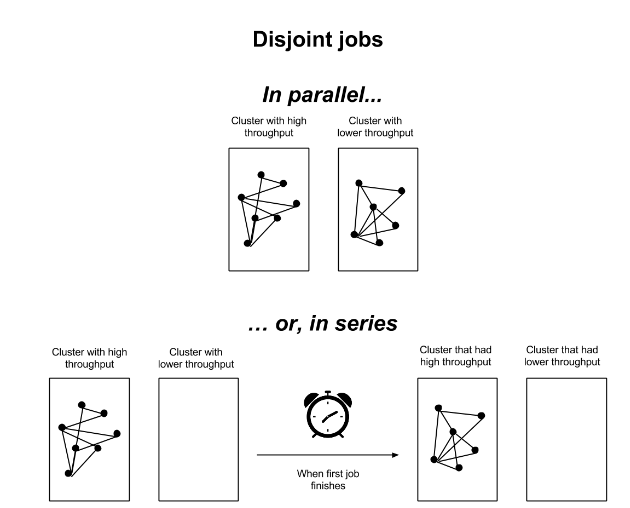
\includegraphics[scale=0.65]{disjointjobs.png}

 \caption{An application that consists of two disjoint jobs.  The vertices represent VMs, and the edges represent communication between VMs within the application.  If we were to run the jobs in series rather than in parallel, the cost might be slightly lower but the time required would be twice as long.}

 \label{fig:disjoint-jobs}
\end{figure}


%\FloatBarrier
\subsubsection{Actively probe network conditions?}

A second trade-off we considered was whether to actively probe network conditions.  Active probing could give us more accurate information about the state of the network, but comes at the cost of increased complexity.  At the root of the matter lies the following question:

\begin{quote}
Is occupancy a good enough heuristic for determining which areas of the network are congested?
\end{quote}

Our answer to this question is yes; the reasoning is as follows.  The typical use case of a data center is traffic-heavy: jobs computed collaboratively by many machines, such as MapReduce.  If there are many VMs in a cluster, it is likely that on average each VM is using a lot of network bandwidth, and thus that the cluster is congested.  Conversely, if there are only a few VMs in a cluster, the load on the network will typically be smaller.  Thus, occupancy is a good heuristic for measuring network congestion in the case of a data center.

We asked whether occupancy is a ``good enough'' heuristic, because there is an alternative.  We could devise a scheme of active probing, in which we send one or more ``scout'' VMs to the different clusters and send artificial data across the network to measure statistics.  This would increase cost, since VM time costs money; the putative benefit would be more accurate measurements of the network conditions.  In our view, the costs outweigh the potential benefits, for the following reasons:

\begin{enumerate}[noitemsep]
  \item For small jobs, active probing would significantly increase the number of running VMs.
  \item Devising rules for active probing adds unnecessary complexity to the system.
  \item Because occupancy is a fairly good heuristic, the marginal gains from active probing would be small.
  \item Measuring occupancy is cheap and fast (a single API call measures the occupancy of a physical machine in the data center).
\end{enumerate}

\subsection{Coordinators}

In addition to the VMs required for the user application, Placr spawns two additional VMs: the \textit{micro coordinator} and the \textit{macro coordinator}.  VMs other than these two coordinators will be referred to as \textit{application VMs}.

The coordinators are the first two VMs spawned by Placr, and are responsible for placing and rearranging application VMs.  The location of the coordinators does not change during the lifetime of the application.  The two coordinators are placed in the same group (or at least, in the same cluster), if such a placement is possible at the time when the application starts.  Each application VM is told the location of the micro coordinator upon initialization.

\subsection{Measurement}

Network statistics are measured in a distributed manner and collected at the micro coordinator.  Each application VM keeps a log of its recent (over the past 100 milliseconds) communications with other VMs.  This logging is done by the network layer of the VM's operating system.  An additional daemon running on each VM periodically reads these logs and generates a summary message called a \textit{report} (see Figure \ref{fig:report}).  Each VM sends a report to the micro coordinator every 100 milliseconds.

The reporting interval of 100 milliseconds was chosen deliberately.  Network usage in the data center changes rapidly enough that a reporting interval on the order of seconds would not provide fresh enough information to make placement decisions upon.  Conversely, a reporting interval of 10 milliseconds or less may ``miss'' important information, if the communication pattern between two VMs is bursty.

\begin{figure}
  \centering
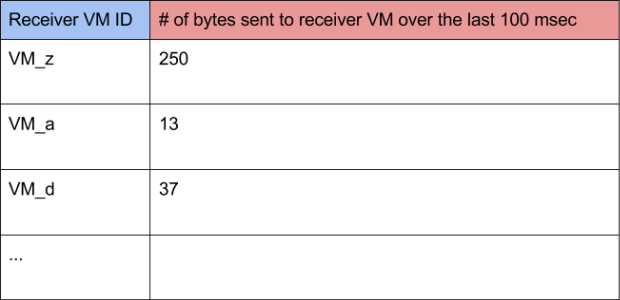
\includegraphics[scale=0.65]{measurement.png}

 \caption{The report data structure for one VM is shown above. Report is an associated array with key, value as follows. key is a VM id that communicated with this VM over the past 100 msec. The associated value is the number of bytes this VM communicated with the VM with id key in the past 100 msec.}
 
 \label{fig:report}
\end{figure}

%\FloatBarrier
\subsection{Placement}

We now give an overview of the placement algorithms used by the micro and macro coordinators.  In the following sections, we describe each of the two algorithms in detail.

\subsubsection{Micro and Macro algorithms}

The micro coordinator runs a fast-paced online algorithm to make small placement decisions as it receives reports from application VMs.  The purpose of this algorithm is to make small, locally optimal choices in order to bring the application's VM placement close to a local optimum.

If the micro coordinator's online algorithm were the only aspect of the placement component, then Placr would run the risk of getting caught in a local optimum that is worse than the global optimum.  For this reason, the placement decisions of the micro coordinator are supplemented by placement decisions of the macro coordinator.  The macro coordinator runs an offline graph algorithm to compute a global rearrangement of all application VMs into available slots in the network.  This computation requires significant computing power and takes a few seconds to complete.  Thus, the macro coordinator works continuously and outputs a placement decision every few seconds.

\subsubsection{Communication between micro and macro coordinators}

The communication between the micro and macro coordinators is as follows.  The micro coordinator forwards all reports it receives to the macro coordinator, in 1-second digests.  The macro coordinator, in turn, sends its placement decisions to the micro coordinator.  The actual execution of the macro coordinator's decisions are carried out by the micro coordinator.  This detail is crucial, as it ensures that only one machine (the micro coordinator) ever executes {\tt place()} API calls.  Therefore, the micro coordinator knows, at all times, the physical location of each VM.  This eliminates the concurrency issues that would arise if multiple machines were moving VMs at the same time.


\subsection{Online algorithm: Micro}
\newcommand{\VMa}{$\textit{VM}_a$}
\newcommand{\VMb}{$\textit{VM}_b$}
Every time a report from a VM is received, the micro coordinator attempts to move that VM, if doing so would decrease the amount of inter-group communication.

If more data is being transferred between a VM (say \VMa) and an external group (say $g$) than between that VM and its own group, then it would be beneficial to move \VMa into group $g$, if there is an open slot (see Figure \ref{fig:micro-move}).  Here, and for the remainder of this section, ``between'' is bidirectional, i.e., is the sum of data sent from \VMa to group $g$ and data sent from group $g$ to \VMa.

\begin{figure}
  \centering
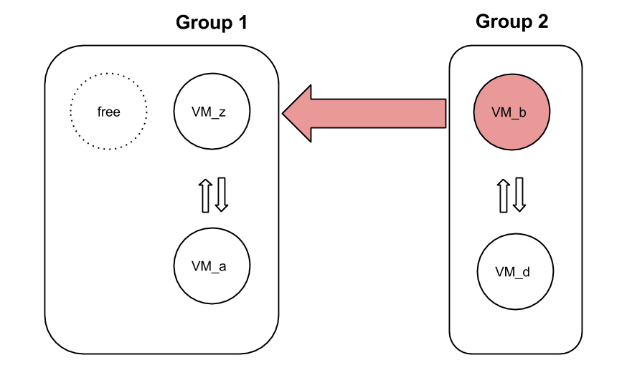
\includegraphics[scale=0.65]{micro1.png}

 \caption{\VMb communicates with group 1 more than its own group.  If there is an open slot, \VMb should be moved to group 1.}

 \label{fig:micro-move}
 
\end{figure}

Even if group $g$ does not have any open slots, it may be beneficial to switch the location of \VMa with one of the VMs in group $g$ (see Figure \ref{fig:micro-switch}).
\begin{figure}
  \centering
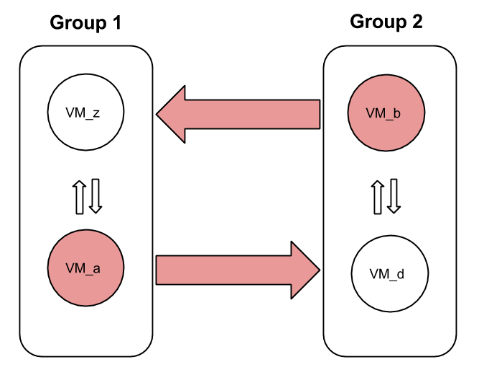
\includegraphics[scale=0.65]{micro2.png}

 \caption{Group 1 and group 2 do not have any open slots, but it would be beneficial to switch the locations of \VMa and \VMb.}

 \label{fig:micro-switch}
 
\end{figure}

To implement the above possibility, the micro-coordinator keeps additional data structures.  For each group, the micro-coordinator stores a ``waiting list'' of VMs that are waiting to move into that group.  (So, there are 24 such lists.)

In the illustration above, the list for group 1 contains \VMb; the list for group 2 contains \VMa.

Here is the algorithm used by the micro coordinator in detail:
\begin{enumerate}
  \item The micro-coordinator receives a report.  Suppose the sender is \VMa.
  \item The micro-coordinator deletes \VMa from any of the 24 lists it is currently on, because \VMa's membership in those lists is now stale.
  \item Based on the report, the micro coordinator computes the total number of bytes sent from \VMa to each group over the past 100 milliseconds.  Let $\texttt{group\_comm}[g]$ be the number of bytes sent from \VMa to group $g$ in the past 100 milliseconds.
  \item Let $g_a$ denote the group in which \VMa currently resides.  For each group g, let
    \[ \texttt{desire\_to\_transfer}[g] = \texttt{group\_comm}[g] - \texttt{group\_comm}[g_a]. \]
    If $\texttt{desire\_to\_transfer}[g] > 0$, then \VMa is transferring more data to group $g$ than to its own group, and thus we should try to move \VMa into group $g$.
  \item For each group $g$ for which $\texttt{desire\_to\_transfer}[g] > 0$, in descending order of the magnitude of $\texttt{desire\_to\_transfer}[g]$, the micro coordinator does the following:
    \begin{enumerate}[label=(\alph{*})]
      \item Use the \texttt{machine\_occupancy()} API call to determine whether there is an open slot in group $g$.  If so, move \VMa into group $g$.
      \item If there are no open slots in group $g$, search through the waiting list for group $g$ to determine whether there is a VM waiting to switch into group $g_a$.  If so, switch the locations of that VM and \VMa.
    \end{enumerate}

  \item If no switch or transfer has yet been made, the micro coordinator adds \VMa to the waiting list of each group $g$ for which $\texttt{desire\_to\_transfer}[g] > 0$.
\end{enumerate}


\FloatBarrier

\subsection{Offline algorithm: Macro}

Every few seconds, the macro coordinator computes a global rearrangement of all the application VMs, and sends it to the micro coordinator to be executed.  We refer to this rearrangement as a macro step.  The efficacy of macro steps relies heavily on the assumption that moving VMs is free, since executing the macro step may require moving many VMs at once.

We now discuss aspects of the macro step in further detail:

\subsubsection{Information used by the macro coordinator}

The macro coordinator uses the following information:

\begin{itemize}
  \item {\em Which VMs are trying to send data to each other.}  Recall that the micro coordinator forwards a copy of all the measurement reports it receives to the macro coordinator in 1-second digests.  This way, the macro coordinator has recent data on which pairs of the user's VMs are transferring data to each other.
    
  \item {\em Which regions of the network are highly occupied.}  The macro coordinator gathers information about the occupancy of each physical machine, using the \texttt{machine\_occupancy()} API call on the physical machines in the cluster.  (There are 1152 physical machines in the cluster; we assume that the network component providing this API can give these 1152 values in, say, under a second.)   We use the occupancy as a heuristic to predict congestion: densely occupied regions are likely to be congested, and sparsely occupied regions are likely to be uncongested.  (See our detailed discussion of this issue above in the \S\ref{sec:tradeoffs}.)  Of course, for purposes of the macro step, slots currently occupied by our own VMs count as open.
\end{itemize}

\subsubsection{Algorithm used to compute the macro step}

The basic problem to be solved by the macro step is as follows.  We wish to find an assignment of VMs to available slots in the data center, such that the amount of communication between groups is minimal and the amount of communication between clusters is minimal.  We first describe the solution of the basic problem; then we discuss two important improvements to the algorithm make it more effective as a VM placement strategy.

We divide the basic problem into two phases. In the first phase, we assign VMs to clusters.  In the second phase, we assign VMs to groups.

To elucidate this process, let us detail the first phase.  Suppose our job requires $n$ VMs.  Let $G$ be a weighted graph with $n$ vertices, with an edge from the $i$th vertex to the $j$th vertex if VM $i$ is trying to transfer data to VM $j$.  The weight assigned to this edge is the number of bytes transferred from machine $i$ to machine $j$ in the past second.  Let $x_k$ be the number of available slots in cluster $k$ ($k = 1,2,3,4$).  Then we face the following graph problem: partition the vertices of $G$ into four disjoint sets $S_1,S_2,S_3,S_4$, such that $|S_k| \leq x_k$, and such that the number of edges crossing from $S_k$ into $S_\ell$ for $k \neq \ell$ is minimized (see Figure \ref{fig:macro-basic-1}).  (The constraint $|S_k| \leq x_k$ says that we can only place as many VMs in cluster $k$ as there are open slots.)  This is the classic Minimum Multicut problem.  Though Minimum Multicut is NP-hard, there exist good approximations which have practical running times.  We use the VMMinKcut algorithm of Meng, Pappas and Zhang \cite{Meng} to solve this instance of Minimum Multicut.  The idea of their algorithm is to use Gomory--Hu trees to make a sequence of greedy choices that leads to a close-to-optimal multicut.

\begin{figure}
  \centering
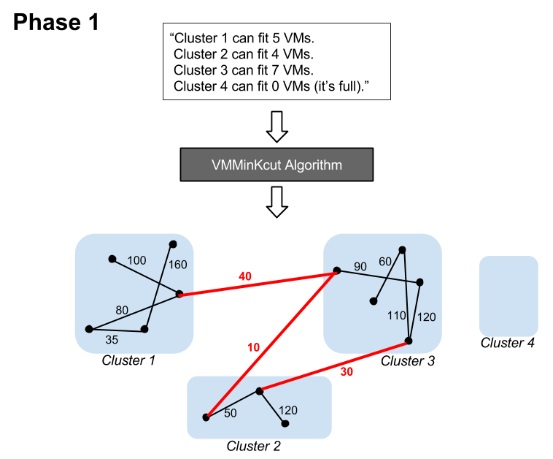
\includegraphics[scale=0.7]{phase1.png}

 \caption{Phase 1 of the basic algorithm.  The maximum sizes of each of the four clusters are specified, and the algorithm finds a configuration in which inter-cluster communication is (approximately) minimized.  In the figure, inter-cluster communication is highlighted in red.}
 
 \label{fig:macro-basic-1}
\end{figure}

The second phase proceeds in exactly the same way.  We have four instances of Minimum Multicut (or fewer, if some of the clusters have not been assigned any VMs by phase one).  Within each cluster, there are six groups.  Let $y_\ell$ be the number of available slots in group $\ell$ ($\ell = 1,\ldots,6)$.  Let $G'$ be the restriction of $G$ to just the vertices corresponding to VMs that have been assigned to the current cluster.  Then we wish to partition the vertices of $G'$ (the virtual machines in the current cluster) into six disjoint sets $S_1, \ldots, S_6$, with $|S_\ell| \leq y_\ell$, such that inter-group communication is minimized.  This is again done using VMMinKcut (see Figure \ref{fig:macro-basic-2}).

\begin{figure}
  \centering
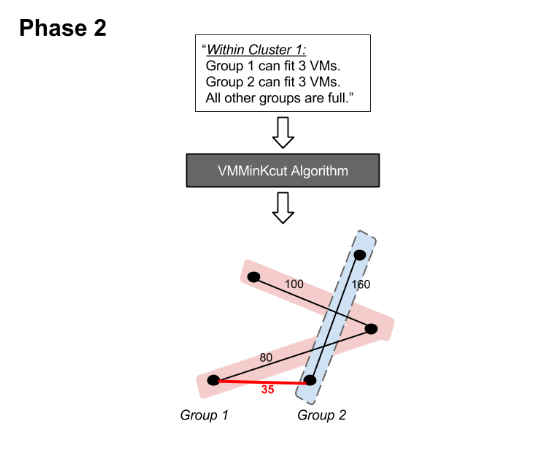
\includegraphics[scale=0.7]{phase2.png}

 \caption{In phase two, we assign the VMs within each cluster to groups.  The number of available slots in each group is specified, and the VMMinKcut algorithm finds an assignment for which inter-group communication is (approximately) minimized.  In the above picture, group 1 is highlighted in pink, group 2 is outlined with a dashed line, and inte-group communication is highlighted in bold red.}
 
 \label{fig:macro-basic-2}

\end{figure}

Once VMs have been assigned to groups, the computation phase of the macro step is complete; the positioning of a VM within its assigned group is arbitrary.  The positioning does not matter because the communication overhead within a group is negligible.

We refer to the above algorithm as the ``basic algorithm.''  The actual algorithm used by the macro coordinator is a modified version of the basic algorithm which incorporates three major improvements.  To motivate these improvements, we first present problems they solve.

\begin{trivlist}
\item \textit{Problem 1}. Because phase one of the basic algorithm considers only clusters and not groups, it is possible that one group within the data center has enough room for all $n$ of our VMs, but we instead assign our VMs to a different cluster in which the open slots are spread out between several groups.  Thus the basic algorithm could lead to suboptimal placement.

\item \textit{Improvement 1}. Before the basic macro step begins, we first check whether there is any one group in the data center with enough open spaces to fit all of our virtual machines.  If there is, we immediately place all our VMs there.  After that, the micro and macro coordinators can be eliminated and VMs can remain where they are until completion of the job.  Since communication overhead within a group is minimal, this is guaranteed to be an optimal placement forever.  Furthermore, if at any point in time all application VMs end up in the same group, the micro and macro coordinators can be eliminated at that time.

\item \textit{Problem 2}. Network conditions are changing.  It is possible that during the few seconds in which we compute the macro step, slots that we thought were available actually got filled up.  Thus, it might not be possible to execute the computed macro step.

\item \textit{Improvement 2}. It is okay if the macro step fails every once in a while; we just need to make sure it does not fail often.  The most likely way in which the macro step could fail is if we plan to use up all available VM slots in a given cluster or group.  Then, if a few new VMs from another user enter the cluster or group, there will not be enough space left to execute our plan.  Thus, we need a way to discourage the basic algorithm from making assignments which use up all the available space in a given cluster or group.

  We achieve this by introducing ``leeway'' to the input to VMMinKcut, in the following way (see Figure \ref{fig:improvements}).  Consider phase one of the basic algorithm (in which VMs are assigned to clusters), and consider a cluster which has $P$ available slots.  Rather than allowing the VMMinKcut algorithm to assign VMs to all $P$ spaces, we allow only at most $P-b$ VMs to be assigned to the cluster.  Here $b$ is the so-called ``leeway.''  Then, as long as not more than $b$ new VMs are added to the cluster during our computation, there will still be enough space to execute the computed macro step.  Thus b should be large enough that, usually, the occupancies of clusters do not change by more than $b$ over the span of a few seconds.  If $b$ is too large, though, we may unnecessarily restrict our choices, forcing ourselves to choose a suboptimal assignment.  We propose the following rule for assigning $b$:

  \begin{quote}
If setting $b=10$ would leave enough room for us to place all $n$ VMs in the network (that is, if the number of available slots in the network is at least $n + 4b$), then we set $b=10$.  Otherwise, we choose the largest value of $b$ that does satisfy this constraint.
  \end{quote}

This leeway strategy applies in the same way to phase two of the basic algorithm (in which we assign VMs to groups), except that the maximum leeway $b$ should be smaller since there are fewer slots in the group.  We propose setting a maximum of $b=5$ in the second phase.  As Placr begins to be used in real data centers, these maximum values of $b$ should be tuned to optimize performance.

\item \textit{Problem 3}. A cluster in which there is one group with lots of open space is preferable to a cluster in which there are several groups each with a little open space, but phase one of the basic algorithm does not take into account the distribution of open space within a cluster.

\begin{figure}
  \centering
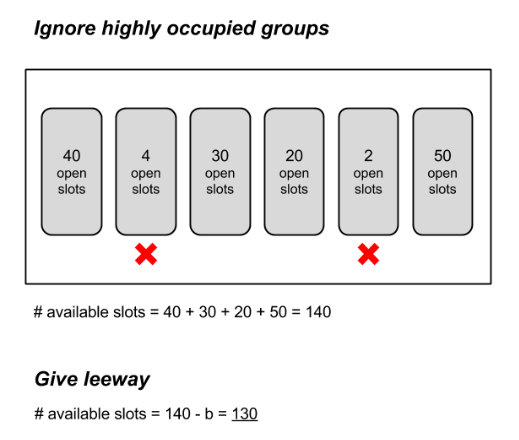
\includegraphics[scale=0.7]{occupiedgroups.png}

 \caption{ Improvements 2 and 3.  To simplify the diagram, we consider only a single cluster, depicted above.  Improvement 3 involves ignoring highly occupied groups.  In the above example, the groups with fewer than 5 available slots are ignored.  Improvement 2 then incorporates a ``leeway'' of $b=10$ to the actual number of available slots.  Ultimately, the number of slots in this cluster made available to the VMMinKcut algorithm is 130.}

 \label{fig:improvements}

\end{figure}

\item \textit{Improvement 3}. The idea is to ``ignore'' groups with high occupancy (see Figure \ref{fig:improvements}).  By ``ignore'' we mean that we treat the ignored group as completely occupied ($y_\ell = 0$), and do not allow VMMinKcut to assign any VMs to it.  The strategy is as follows.  We set a parameter $c$ (which can be tuned; a reasonable starting point would be $c=5$).  Then:

\begin{itemize}
  \item Pick a group with fewer than $c$ open slots.  If, after ignoring this group, there are still $n$ available VM slots, then ignore the group.
  \item Repeat this process until all groups have at least $c$ open slots, or until ignoring another group would result in fewer than $n$ available VM slots.
\end{itemize}

This improvement encourages phase one to favor clusters in which there are groups with lots of open space.  It also discourages assignment to congested clusters, since the groups in such clusters will not have much open space.

\end{trivlist}

\FloatBarrier
\section{Analysis}

In this section, we'll look at a few of the common use cases of Placr and how it performs in each.  We'll be looking at varying levels of occupancy, job size, job arrival rate in the data center, and strategies used by other users.

\subsection{Low Number of VMs}

A job with a low number of VMs is the most basic use case of the system.  Unless the data center is very highly occupied, all application VMs will be placed in the same group and the coordinators will shut down for the remainder of the application.

If there is not enough space for all our VMs in any one group, the macro coordinator will determine a placement of our VMs that minimizes inter-group communication.  If at a later time a group recovers enough free space to fit all our application VMs, our application VMs will be moved to that group and stay there.

The overhead of having two extra VMs for coordination may be undesirable in the case of a small application.  If this use case turns out to be common, the system will need modifications.

\subsection{High Number of VMs, Many Open Slots}

Placr should effectively handle the case of high number of VMs, many open slots.  By ``many'' we mean that the data center has significantly more slots open than the job requires. In general, our two-level macro placement strategy should place the VMs close to each other with minimal inter-group and inter-cluster communication.  Our special rule to first check if all machines can be in the same group will produce an extremely efficient placement if the check succeeds.  If a group with enough occupancy for the whole system exists, Placr will use it.

There may be times when the clustering by phase one of the macro step is suboptimal. For example, if one cluster has two groups which are empty, and another cluster has four groups which are about half full, our system will treat both clusters as if they have the same occupancy in phase one of the macro step. However, dividing VMs between two groups is significantly better than dividing into four groups, so the first cluster should have been favored. This problem is partially, but not entirely, alleviated by improvement 3 of the macro step: very highly occupied groups are ignored, but half-full groups are not distinguished from very unoccupied groups.

In a use case where there are many application VMs, the overhead of having two additional VMs as coordinators is not significant.  VM throughput is maximized, so time and cost should both be close to optimal.


\subsection{High Number of VMs, Few Open Slots}

The case of high number of VMs with few open slots was the most difficult case considered during the design of Placr.  The job will be spread across several groups and clusters and our goal is to minimize the network traffic across routers.  We believe that Placr should perform very well in this case though.

The first level of clustering places VMs into clusters such that inter-cluster communication is minimal.  It is unlikely that any one group will have enough space for many VMs, so minimizing inter-group communication is more important.  Our two-phase macro clustering algorithm should be very effective at this, since the algorithm focuses more on minimizing intercommunication than on creating large groups.

Micro optimizations will be especially helpful in this case, since it is likely that many of the groups will have significant inter-group communication.  Micro optimizations will be able to react to changing data transfer characteristics and quickly adjust the VM placement to avoid inter-group communication.  Since more data flows between groups in this case, we expect that more adjustments will be made by the micro coordinator.

Due to micro-adjustments, our system should be very effective at navigating this highly constrained environment to keep time low.  As in the previous case, the cost of having two extra VMs as coordinators is insignificant.


\subsection{Competing Placements}

We must also consider the situation when there are many applications using Placr as their placement strategy.  In this case, everyone would be trying to use macro optimizations to improve their position in the network.  In this case, we would expect much more movement across the network, which could cause problems for our macro optimizations.

Situations such as a job finishing and many VMs leaving the network could result in a race by all other users to fill the empty space.  Figure \ref{fig:macrodelay} illustrates a problematic situation that we could encounter.

\begin{figure}
  \centering
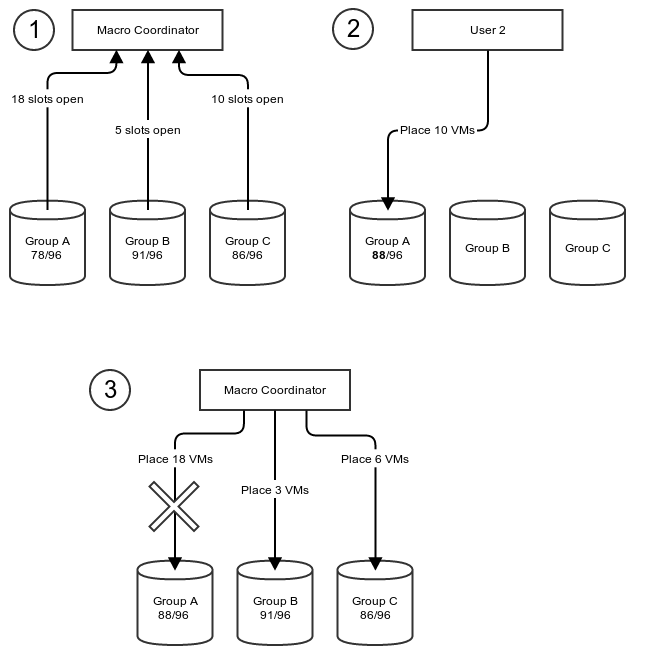
\includegraphics[scale=0.65]{macrodelay.png}

 \caption{In step 1, the macro coordinator collects information on group occupancy.  Next, in step 2, another user places 10 VMs in group A, decreasing the occupancy.  Finally, in step 3, the macro coordinator tries to execute the placements it calculated and place 18 VMs in group A.  Unfortunately, since another user already placed 10 VMs in group A, the placement the macro coordinator calculated is invalid.}

 \label{fig:macrodelay}
 
\end{figure}

It seems correct, however, to take part in this race. If we are able to succeed and take the spot, then we'll benefit from our improved position.  It's clear that if our macro optimization steps are failing often, we aren't getting the best possible position though.  That is why we have added leeway into our macro step.  By assuming fewer open positions exist than are truly available, we account for changes in occupancy due to competing users. While we still expect the macro step to fail occasionally, the problem should be somewhat alleviated. 

Our strategy is better optimized for situations where other users are using ``dumb'' strategies, but we still handle competitive cases as well. We will be slightly less efficient in time and cost, but this is expected when the competition for good locations is higher.

\subsection{High rate of Job Arrival}

Data centers with high rates of job arrivals are similar to the case of users with competitive strategies.  Because the occupancies of slots will be changing rapidly, the macro step is liable to fail occasionally, as new jobs can occupy the old spots during the time it takes to complete macro step. The leeway added during the macro step should help us navigate this situation just as it did in the competitive case.

Incoming jobs from other users will likely cause sharp increases in intercommunication, if the computation is spread across multiple groups and clusters.  The micro-adjustments will react to this to some extent, but a macro step is crucial to achieving low time and cost.  If the typical job arrival rate is so fast that the macro step fails with high frequency, modifications to Placr will be necessary.

\section{Areas for Improvement}

While we believe our system as it stands is very strong, we have also identified several areas in which it could be improved.

\subsection{Network Congestion}

One of the first areas in which we see room for improvement is in our use of network congestion information. Although we do attempt to minimize communication between our own VMs, we do not directly take into account congestion caused by other users.  One situation in which this could be relevant is if there is another application that is sending a large amount of data through the aggregator, making it undesirable to be in the same cluster as that application.

For example, in Figure \ref{fig:cluster_congestion}, Clusters 1 and 4 are fully saturating their links to an aggregator, while clusters 2 and 3 have minimal inter-cluster communication.

\begin{figure}
  \centering
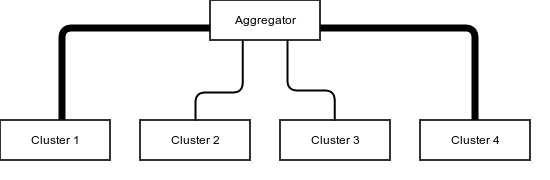
\includegraphics[scale=0.7]{cluster_congestion.png}

 \caption{Line thickness indicates magnitude of data transfer.}

 \label{fig:cluster_congestion}
 
\end{figure}
 
 In this situation, it is preferable to place VMs in clusters 2 and 3 if the job is large enough that inter-cluster communication is required.  In the current design however, all clusters are treated equally if they have the same levels of occupancy.
 
\subsection{Progress}

As it stands, Placr does not use the matrix B, which tells us how much data each VM is expected to transfer to each other VM. We are more concerned about instantaneous data transfer rates since machines can be moved so quickly and cheaply.  Occasionally, however, it is better to make sacrifices in instantaneous data transfer to ensure that a VM completes its entire job faster.  Once a VM completes its job, we can remove it from the network so that it does not take spaces that other VMs could be using.  After this machine is removed, we can place the remaining machines more optimally.

One idea we considered to fix this was to inflate the data transfer measurements from VMs that have made little progress so far.  Since our algorithm minimizes intercommunication, it would be more likely to generate a placement that is favorable to the VMs that have made little progress, allowing them to ``catch up.''  The rate of inflation is a parameter that could be tuned by testing in a real data center.

In addition, we would have to expand our notion of progress beyond the \texttt{progress()} API function since we are concerned about both data transfer into the VM, and out to other VMs.  A VM that is finished sending data, but only half way done receiving data needs to be treated differently than a VM that has both finished sending data and receiving data.  We believe this is a solvable problem, though it needs further study.

\section{Conclusion}

Placr is an effective system for placing VMs within a data center, under the assumption that VMs can be moved quickly and cheaply.  Throughput reports from VMs, a two level macro placement algorithm, and hill-climbing micro optimizations combine to achieve low time and cost of the user's application.  In the most common situations, we expect our system to find a close to optimal placement. For the edge cases where we believe Placr is currently inefficient, we have proposed possible solutions and areas for further study.



\begin{thebibliography}{9}

\bibitem{Meng}
  X. Meng, V. Pappas, and L. Zhang, ``Improving the scalability of data
center networks with traffic-aware virtual machine placement,'' in IEEE
INFOCOM, 2010.

\bibitem{MengSlides}
X. Meng, V. Pappas, and L. Zhang, Alexey Yarovinsky ``Improving the scalability of data
center networks with traffic-aware virtual machine placement,'' [Online Document] [cited 2014 May 11], Available HTTP: http://cs.engr.uky.edu/~qian/CS685/TVMPP.pdf.

\bibitem{Piazza}
 Pratiksha Thaker ``Cost of moving a VM?,'' [Online Document] [cited 2014 May 11], Available HTTP: https://piazza.com/class/hp4dt9k35qp33s?cid=415.

\end{thebibliography}

\end{document}



